%
%Не забыть:
%--------------------------------------
%Вставить колонтитулы, поменять название на титульнике



%--------------------------------------

\documentclass[a4paper, 12pt]{article} 

%--------------------------------------
%Russian-specific packages
%--------------------------------------
%\usepackage[warn]{mathtext}
\usepackage[T2A]{fontenc}
\usepackage[utf8]{inputenc}
\usepackage[english,russian]{babel}
\usepackage[intlimits]{amsmath}
\usepackage{esint}
%--------------------------------------
%Hyphenation rules
%--------------------------------------
\usepackage{hyphenat}
\hyphenation{ма-те-ма-ти-ка вос-ста-нав-ли-вать}
%--------------------------------------
%Packages
%--------------------------------------
\usepackage{amsmath}
\usepackage{amssymb}
\usepackage{amsfonts}
\usepackage{amsthm}
\usepackage{latexsym}
\usepackage{mathtools}
\usepackage{etoolbox}%Булевые операторы
\usepackage{extsizes}%Выставление произвольного шрифта в \documentclass
\usepackage{geometry}%Разметка листа
\usepackage{indentfirst}
\usepackage{wrapfig}%Создание обтекаемых текстом объектов
\usepackage{fancyhdr}%Создание колонтитулов
\usepackage{setspace}%Настройка интерлиньяжа
\usepackage{lastpage}%Вывод номера последней страницы в документе, \lastpage
\usepackage{soul}%Изменение параметров начертания
\usepackage{hyperref}%Две строчки с настройкой гиперссылок внутри получаеммого
\usepackage[usenames,dvipsnames,svgnames,table,rgb]{xcolor}% pdf-документа
\usepackage{multicol}%Позволяет писать текст в несколько колонок
\usepackage{cite}%Работа с библиографией
\usepackage{subfigure}% Человеческая вставка нескольких картинок
\usepackage{tikz}%Рисование рисунков
\usetikzlibrary{circuits} % подключаем библиотеки, содержащие
\usetikzlibrary{circuits.ee} % УГО для схем
\usetikzlibrary{circuits.ee.IEC}
\usetikzlibrary{arrows} % подключаем библиотеки со стрелками
\usetikzlibrary{patterns} % и со штриховкой
\usepackage{float}% Возможность ставить H в положениях картинки
% Для картинок Моти
\usepackage{misccorr}
\usepackage{lscape}
\usepackage{cmap}
\usepackage{bm}



\usepackage{graphicx,xcolor}
\graphicspath{{Pictures/}}
\DeclareGraphicsExtensions{.pdf,.png,.jpg}

%----------------------------------------
%Список окружений
%----------------------------------------
\newenvironment {theor}[2]
{\smallskip \par \textbf{#1.} \textit{#2}  \par $\blacktriangleleft$}
{\flushright{$\blacktriangleright$} \medskip \par} %лемма/теорема с доказательством
\newenvironment {proofn}
{\par $\blacktriangleleft$}
{$\blacktriangleright$ \par} %доказательство
%----------------------------------------
%Список команд
%----------------------------------------
\newcommand{\grad}
{\mathop{\mathrm{grad}}\nolimits\,} %градиент

\newcommand{\diver}
{\mathop{\mathrm{div}}\nolimits\,} %дивергенция

\newcommand{\rot}
{\ensuremath{\mathrm{rot}}\,}

\newcommand{\Def}[1]
{\underline{\textbf{#1}}} %определение

\newcommand{\RN}[1]
{\MakeUppercase{\romannumeral #1}} %римские цифры

\newcommand {\theornp}[2]
{\textbf{#1.} \textit{ #2} \par} %Написание леммы/теоремы без доказательства

\newcommand{\qrq}
{\ensuremath{\quad \Rightarrow \quad}} %Человеческий знак следствия

\newcommand{\const}{\text{const}} % Написание const в формулах

\newcommand{\qlrq}
{\ensuremath{\quad \Leftrightarrow \quad}} %Человеческий знак равносильности

\renewcommand{\phi}{\varphi} %Нормальный знак фи

\renewcommand{\epsilon}{\varepsilon}

\newcommand{\me}
{\ensuremath{\mathbb{E}}}

\newcommand{\md}
{\ensuremath{\mathbb{D}}}



%\renewcommand{\vec}{\overline}




%----------------------------------------
%Разметка листа
%----------------------------------------
\geometry{top = 3cm}
\geometry{bottom = 2cm}
\geometry{left = 1.5cm}
\geometry{right = 1.5cm}
%----------------------------------------
%Колонтитулы
%----------------------------------------
\pagestyle{fancy}%Создание колонтитулов
\fancyhead{}
%\fancyfoot{}
\fancyhead[R]{\textsc{Экзамен. Оптика}}%Вставить колонтитул сюда
%----------------------------------------
%Интерлиньяж (расстояния между строчками)
%----------------------------------------
%\onehalfspacing -- интерлиньяж 1.5
%\doublespacing -- интерлиньяж 2
%----------------------------------------
%Настройка гиперссылок
%----------------------------------------
\hypersetup{				% Гиперссылки
	unicode=true,           % русские буквы в раздела PDF
	pdftitle={Заголовок},   % Заголовок
	pdfauthor={Автор},      % Автор
	pdfsubject={Тема},      % Тема
	pdfcreator={Создатель}, % Создатель
	pdfproducer={Производитель}, % Производитель
	pdfkeywords={keyword1} {key2} {key3}, % Ключевые слова
	colorlinks=true,       	% false: ссылки в рамках; true: цветные ссылки
	linkcolor=blue,          % внутренние ссылки
	citecolor=blue,        % на библиографию
	filecolor=magenta,      % на файлы
	urlcolor=cyan           % на URL
}
%----------------------------------------
%Работа с библиографией (как бич)
%----------------------------------------
\renewcommand{\refname}{Список литературы}%Изменение названия списка литературы для article
%\renewcommand{\bibname}{Список литературы}%Изменение названия списка литературы для book и report
%----------------------------------------
\begin{document}
	\begin{titlepage}
		\begin{center}
			$$$$
			$$$$
			$$$$
			$$$$
			{\Large{НАЦИОНАЛЬНЫЙ ИССЛЕДОВАТЕЛЬСКИЙ УНИВЕРСИТЕТ}}\\
			\vspace{0.1cm}
			{\Large{ВЫСШАЯ ШКОЛА ЭКОНОМИКИ}}\\
			\vspace{0.25cm}
			{\large{Факультет физики}}\\
			\vspace{5.5cm}
			{\Huge\textbf{{Экзамен}}}\\%Общее название
			\vspace{1cm}
			{\LARGE{<<Оптика>>}}\\%Точное название
			\vspace{2cm}
			\vfill
			\includegraphics[width = 0.2\textwidth]{HSElogo}\\
			\vfill
			Москва\\
			2020
		\end{center}
	\end{titlepage}
	
	\tableofcontents
	
	\newpage
	
	\input{TeX_files/1.tex}
	
	\newpage
	
	%
%Не забыть:
%--------------------------------------
%Вставить колонтитулы, поменять название на титульнике



%--------------------------------------

\documentclass[a4paper, 12pt]{article} 

%--------------------------------------
%Russian-specific packages
%--------------------------------------
%\usepackage[warn]{mathtext}
\usepackage[T2A]{fontenc}
\usepackage[utf8]{inputenc}
\usepackage[english,russian]{babel}
\usepackage[intlimits]{amsmath}
\usepackage{esint}
%--------------------------------------
%Hyphenation rules
%--------------------------------------
\usepackage{hyphenat}
\hyphenation{ма-те-ма-ти-ка вос-ста-нав-ли-вать}
%--------------------------------------
%Packages
%--------------------------------------
\usepackage{amsmath}
\usepackage{amssymb}
\usepackage{amsfonts}
\usepackage{amsthm}
\usepackage{latexsym}
\usepackage{mathtools}
\usepackage{etoolbox}%Булевые операторы
\usepackage{extsizes}%Выставление произвольного шрифта в \documentclass
\usepackage{geometry}%Разметка листа
\usepackage{indentfirst}
\usepackage{wrapfig}%Создание обтекаемых текстом объектов
\usepackage{fancyhdr}%Создание колонтитулов
\usepackage{setspace}%Настройка интерлиньяжа
\usepackage{lastpage}%Вывод номера последней страницы в документе, \lastpage
\usepackage{soul}%Изменение параметров начертания
\usepackage{hyperref}%Две строчки с настройкой гиперссылок внутри получаеммого
\usepackage[usenames,dvipsnames,svgnames,table,rgb]{xcolor}% pdf-документа
\usepackage{multicol}%Позволяет писать текст в несколько колонок
\usepackage{cite}%Работа с библиографией
\usepackage{subfigure}% Человеческая вставка нескольких картинок
\usepackage{tikz}%Рисование рисунков
\usepackage{float}% Возможность ставить H в положениях картинки
% Для картинок Моти
\usepackage{misccorr}
\usepackage{lscape}
\usepackage{cmap}



\usepackage{graphicx,xcolor}
\graphicspath{{Pictures/}}
\DeclareGraphicsExtensions{.pdf,.png,.jpg}

%----------------------------------------
%Список окружений
%----------------------------------------
\newenvironment {theor}[2]
{\smallskip \par \textbf{#1.} \textit{#2}  \par $\blacktriangleleft$}
{\flushright{$\blacktriangleright$} \medskip \par} %лемма/теорема с доказательством
\newenvironment {proofn}
{\par $\blacktriangleleft$}
{$\blacktriangleright$ \par} %доказательство
%----------------------------------------
%Список команд
%----------------------------------------
\newcommand{\grad}
{\mathop{\mathrm{grad}}\nolimits\,} %градиент

\newcommand{\diver}
{\mathop{\mathrm{div}}\nolimits\,} %дивергенция

\newcommand{\rot}
{\ensuremath{\mathrm{rot}}\,}

\newcommand{\Def}[1]
{\underline{\textbf{#1}}} %определение

\newcommand{\RN}[1]
{\MakeUppercase{\romannumeral #1}} %римские цифры

\newcommand {\theornp}[2]
{\textbf{#1.} \textit{ #2} \par} %Написание леммы/теоремы без доказательства

\newcommand{\qrq}
{\ensuremath{\quad \Rightarrow \quad}} %Человеческий знак следствия

\newcommand{\const}{\text{const}} % Написание const в формулах

\newcommand{\qlrq}
{\ensuremath{\quad \Leftrightarrow \quad}} %Человеческий знак равносильности

\renewcommand{\phi}{\varphi} %Нормальный знак фи

\newcommand{\me}
{\ensuremath{\mathbb{E}}}

\newcommand{\md}
{\ensuremath{\mathbb{D}}}



%\renewcommand{\vec}{\overline}




%----------------------------------------
%Разметка листа
%----------------------------------------
\geometry{top = 3cm}
\geometry{bottom = 2cm}
\geometry{left = 1.5cm}
\geometry{right = 1.5cm}
%----------------------------------------
%Колонтитулы
%----------------------------------------
\pagestyle{fancy}%Создание колонтитулов
\fancyhead{}
%\fancyfoot{}
\fancyhead[R]{\textsc{Экзамен. Оптика}}%Вставить колонтитул сюда
%----------------------------------------
%Интерлиньяж (расстояния между строчками)
%----------------------------------------
%\onehalfspacing -- интерлиньяж 1.5
%\doublespacing -- интерлиньяж 2
%----------------------------------------
%Настройка гиперссылок
%----------------------------------------
\hypersetup{				% Гиперссылки
	unicode=true,           % русские буквы в раздела PDF
	pdftitle={Заголовок},   % Заголовок
	pdfauthor={Автор},      % Автор
	pdfsubject={Тема},      % Тема
	pdfcreator={Создатель}, % Создатель
	pdfproducer={Производитель}, % Производитель
	pdfkeywords={keyword1} {key2} {key3}, % Ключевые слова
	colorlinks=true,       	% false: ссылки в рамках; true: цветные ссылки
	linkcolor=blue,          % внутренние ссылки
	citecolor=blue,        % на библиографию
	filecolor=magenta,      % на файлы
	urlcolor=cyan           % на URL
}
%----------------------------------------
%Работа с библиографией (как бич)
%----------------------------------------
\renewcommand{\refname}{Список литературы}%Изменение названия списка литературы для article
%\renewcommand{\bibname}{Список литературы}%Изменение названия списка литературы для book и report
%----------------------------------------

\begin{document}
	\section{Явление полного внутреннего отражения, его применения. Оптические элементы и
		приборы, работающие на явлении полного внутреннего отражения. Оптоволокно,
		типы оптоволокна.}
	Сначала наивное. Мы знаем формулу Снеллиуса $\sin \theta = n_{21} \sin \theta'$, где $n_{21}$ -- это относительная оптическая плотность. Если $n_{21} < 1$ то должен существовать такой угол падения $\arcsin n_{21}$ после которого не может уже существовать никакого прошедшего луча, а только отраженный. Так как свету некуда деться, кроме как отразиться, то он отражается полностью. 
	
	Теперь как это выглядит с точки зрения волновой оптики (Сивухин с 402)\\
	Пусть у нас есть падающая волна:
	\begin{align*}
		E^{e} = \mathcal{E} e^{i(\omega t - k_1 r)}
	\end{align*}
	Мы из соображений геометрической оптики знаем, что должны быть еще отраженная (r) и прошедшая (d) волны:
	\begin{align*}
	E^{r} = \mathcal{R} e^{i(\omega t - k'_1 r)}\\E^{d} = \mathcal{D} e^{i(\omega t - k_2 r)}
	\end{align*}
	Мы предполагаем что они тоже плоские из соображений симметрии. Равенство частот у всех трех объясняется тем, что напряженности могут иметь только гармоническую зависимость от времени, а в случае наложения двух плоских полей с разными частотами такое не выполняется.\\
	Из соотношений симметрии надо заключить, что касательная к плоскости составляющая волнового вектора у всех трех волн одинаковая. В нашем случае это проекция на ось x (смотри рисунок)
	\begin{figure}[H]
		\includegraphics*[scale = 0.3]{2_1}
	\end{figure}
	То есть: $k_{1x} = k'_{1x} = k_{2x}$\\
	Так же можем написать про волновые вектора:
	\begin{align*}
	k_1^2 = k_1'^2 = \dfrac{\omega^2 }{c^2 } \varepsilon_1\\
	k_2^2 = \dfrac{\omega^2 }{c^2 } \varepsilon_2
	\end{align*}
	Где эпсилон 1 и 2 это диэлектрическая проницаемость среды из которой пришел луч и в которую ушел соответственно. Отсюда можно узнать их z составляющие:
	\begin{align*}
	k'_{1z} = - \sqrt{k_1^2 - k_{1x}^2}\\
	k_{2z} = \sqrt{k_2^2 - k_{1x}^2}	
	\end{align*}
	Так как нас волнует полное внутреннее отражение, то рассмотрим случай, когда $k_2^2 < k_{1x}^2 $ так как $k_{1x} = k_1 \sin \phi$, то это условие равносильно условию $\sin \phi > \sqrt{\dfrac{\varepsilon_2}{\varepsilon_1}} = n_{21}$ так же как в геометрической оптике. Естественно чтобы такое условие вообще могло выполняться надо чтобы $n_{21}<1$. В этом случае $k_{2z}$ комплексный. Обозначим так: $k_{2z} = \dfrac{-i}{2h}$ Почему минус? Потому что корень это функция многозначная и нужную ветвь мы выбираем исходя из физических требований, а тут нужен как раз минус. Со всем этим можем написать отраженную волну как:
	\begin{align*}
	E^{d} = \mathcal{D}e^{-z/2h} e^{i(\omega t - k_{1x} x)}\\
	h = \dfrac{\lambda_1}{4\pi \sqrt{\sin^2 \phi  - n_{21}^2}}
	\end{align*}
	То есть волна идет вдоль границы, но затухает вглубь вещества (см рисунок)
	\begin{figure}[H]
		\centering
		\caption{Опыт Мандельштама и Селени}
		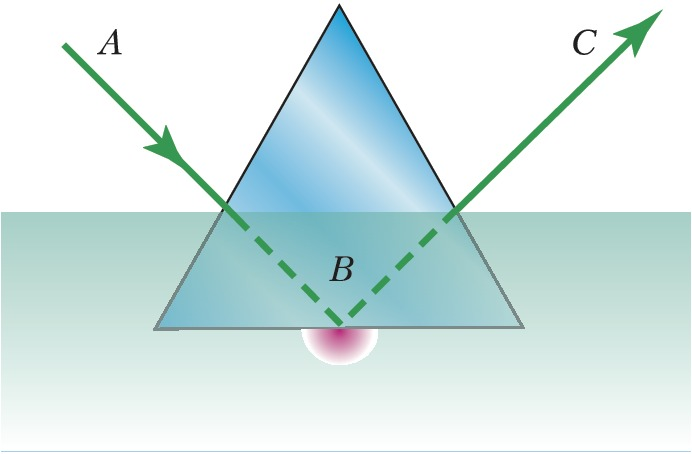
\includegraphics[scale = 1]{2_2}
	
	\end{figure}
	Эффект полного внутреннего отражения используется например в уголковых отражателях и во многих других призмах:
		\begin{figure}[H]
			\centering
			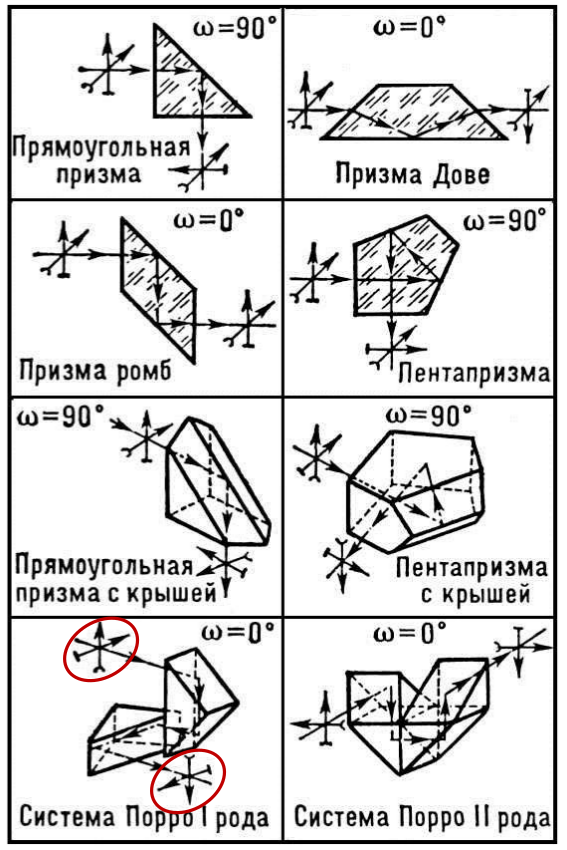
\includegraphics[scale = 0.3]{2_3}
		\end{figure}
	Оптоволокно это такая штука, в которой свет постоянно испытывает отражения от стенок. Состоит из двух слоев очевидно. Внешний имеет оптическую плотность больше. Заодно он защищает внутренний слой от повреждений. Сгибать сильно нельзя.
\end{document}
	
	\newpage
	
	\section{Преломление на сферической поверхности. Фокусы сферичекой поверхности. Изображение предмета. Преломление в линзе. Общая формула линзы (вывод). Фокусные расстояния тонкой линзы. Действительное и мнимое изображения. Линейное (поперечное) увеличение. Оптическая сила линз.}

Сначала введём необходимые определения:
\begin{enumerate}

\item{\textbf{Оптическая система} — совокупность оптических элементов (преломляющих, отражающих), созданная для преобразования световых пучков.}

\item{\textbf{Оптическая ось системы} — прямая линия, являющаяся осью симметрии преломляющих (отражающих) поверхностей. Она проходит перпендикулярно этим поверхностям через их центр кривизны.}

\item{\textbf{Центрированная оптическая система} — совокупность однородных преломляющих и отражающих сред, отделённых друг от друга симметричными поверхностями, центры кривизны которых находятся на одной прямой. Эту прямую называют \textit{главной оптической осью системы}.}

\item{\textbf{Гомоцентрический пучок} — пучок, все образующие лучи которого при своём продолжении сходятся в одной точке. \textit{Параллельный} пучок тоже считается гомоцентрическим, т.к. он исходит из бесконечно удалённой точки.}

\item{\textbf{Параксиальный пучок} — пучок, все образующие лучи которого распространяются вдоль оси центрированной оптической системы и образуют малые углы с осью и нормалями к преломляющим и отражающим поверхностям.}

\item{Пусть оптическая система преобразует свет, не нарушая гомоцентричности пучка, причём пучок лучей, исходящий из точки $P$, сходится в точке $P'$. Тогда точка $P'$ — это \textbf{изображение} точки $P$.}


\item{Изображение называется \textbf{действительным}, если световые лучи от точки $P$ сходятся к точке $P'$ при своём распространении. Если же в точке $P'$ сходятся продолжения лучей в направлении, обратном направлению распространения света, то изображение называется \textbf{мнимым}.}

\item{Пусть  на  оптическую  систему  падает  пучок  лучей, параллельных  главной  оптической  оси.  \textbf{Задний (второй главный) фокус} -- это точка пересечения пучка таких лучей (или их  продолжений)  на  выходе  из  системы.}

\item{Если на систему падает  пучок лучей, исходящий из некоторой  точки,  и  после  прохождения  оптической  системы  лучи  идут параллельно главной оптической оси, исходная точка называется \textbf{передним (первым главным) фокусом}. Передний и задний фокусы всегда лежат на главной оптической оси.}

\item{\textbf{Линейное (поперечное) увеличение} — отношение линейных размеров изображения и предмета:
\begin{equation}
\beta = \frac{y'}{y}.
\label{eq:lin_magn}
\end{equation} 

Отрезки $y$ и $y'$ считаеются положительными, если они откладываются вверх от оптической оси, и отрицательными — в противном случае.}

\item{Если увеличение положительное, то изображение \textbf{прямое}. В противном случае изображение \textbf{обратное}.}

\item{Две сопряжённые плоскости, отображающиеся с линейным увеличением $\beta = 1$, называются \textit{главными}. Точки пересечения главных плоскостей с главной оптической осью — \textit{главные точки} оптической системы.}

\item{\textbf{Главные фокусные расстояния} — расстояния от главных точек до соответствующих фокусов. Эти расстояния считаются положительными, если свет идёт от главной плоскости к соответствующему главному фокусу (правило знаков).}


\end{enumerate}

\subsection{Преломление на сферической поверхности}
 
Пусть две среды с разными показателями преломления ($n$ и $n'$) отделены друг от друга сферической границей $S$ радиуса $R$. Эта граница может рассматриваться как оптическая система, преобразующая падающее на неё излучение предмета. Считаем радиус сферы положительным, если её центр находится с той стороны, куда распространяются лучи.

\begin{figure}[H]
	\centering
	\includegraphics*[width=0.7\textwidth]{3_1}
\end{figure}


Рассмотрим луч $OP$, выходящий из точки $O$, испытывающий преломление в точке $P$ и пересекающий оптическую ось в точке $O'$. Проведём из центра сферы радиус $CP$. Он ортогонален поверхности сферы $S$, так что для углов $\alpha$ и $\beta$ можно записать закон Снеллиуса:

\begin{equation}
n \sin{\alpha} = n' \sin{\beta}.
\label{eq:snellius_sphere}
\end{equation} 

Обозначим путь луча $OP$ как $u$, а дальнейший путь $PO'$ как $u'$. Найдём их связь из геометрических соображений:

\begin{equation*}
S_{OPC} + S_{PCO'} = S_{O'PO},
\end{equation*}

\begin{align*}
S_{OPC} = -\frac{1}{2}& uR \sin{\alpha}, \\ 
S_{PCO'} = \frac{1}{2}&u'R\sin{\beta}, \\
S_{O'PO} = -\frac{1}{2}&uu'\sin{(\pi - \alpha + \beta).}
\end{align*} 

Из этих равенств находим

\begin{equation*}
-uR\sin{\alpha} + u'R\sin{\beta} = -uu'\sin{(\alpha - \beta).}
\end{equation*}

Подставляем (\ref{eq:snellius_sphere}) и находим

\begin{equation*}
-u + u'\frac{n}{n'} = -\frac{uu'}{R}\Big(\cos{\beta} - \cos{\alpha} \frac{n}{n'}\Big),
\end{equation*}

или

\begin{equation}
\frac{n}{u} - \frac{n'}{u'} = \frac{n\cos{\alpha} - n'\cos{\beta}}{R}.
\label{eq:spherical_surface}
\end{equation}

Это точное соотношение. В случае параксиальных пучков, для которых $|\alpha| \ll 1$, $|\beta| \ll 1$, формула (\ref{eq:spherical_surface}) принимает вид

\begin{equation}
\frac{n}{x} - \frac{n'}{x'} = \frac{n - n'}{R},
\label{eq:spherical_surface1}
\end{equation}

где $x$ — расстояние от точки $O$ до поверхности сферы, $x'$ — расстояние от точки $O'$ до поверхности сферы. Знаки величин $x$ и $x'$ определяются так же, как и для $u$ и $u'$, из того условия, что отсчёт расстояния ведётся от преломляющей поверхности \textit{по направлению лучей}.

Подставив $x = -\infty$ и $x' = \infty$, находим положение заднего и переднего фокусов соответственно:

\begin{align*}
 f' = x' = &\frac{R}{1 - n/n'}, \\ 
 f = x = -R&\frac{n/n'}{1 - n/n'}. \\
\end{align*} 

\subsection{Тонкие линзы}

\textbf{Линза} — это прозрачное тело, изготовленное из прозрачного оптически однородного материала, ограниченное двумя полированными выпуклыми или вогнутыми поверхностями. 

Точки пересечения поверхностей линзы с оптической осью называются \textit{вершинами линзы}. Расстояние $d$ между вершинами линзы называется \textit{толщиной линзы}. Линза считается \textbf{тонкой}, если её толищина мала по сравнению с радиусами кривизны поверхностей: $d \ll R_{1}$, $d \ll R_{2}$. Главные плоскости тонкой линзы совпадают.

Представим линзу как совокупность двух последовательных преломляющих поверхностей. Согласно (\ref{eq:spherical_surface1}), для первой поверхности имеем:

\begin{equation*}
\frac{n_{e}}{x} - \frac{n_{i}}{x_{1}} = \frac{n_{e} - n_{i}}{R_{1}}.
\end{equation*}

Поскольку линза предполагается тонкой, то координата $x_{1}$ промежуточного изображения одинакова относительно обеих поверхностей. Следовательно, для второй поверхности можем записать

\begin{equation*}
\frac{n_{i}}{x_{1}} - \frac{n_{e}}{x'} = \frac{n_{i} - n_{e}}{R_{2}}.
\end{equation*}

Складывая эти равенства, получаем 

\begin{equation}
\frac{1}{x} - \frac{1}{x'} = -(n - 1) \Big(\frac{1}{R_{1}} - \frac{1}{R_{2}}\Big),
\label{eq:lens_formula}
\end{equation}

Здесь мы перешли к относительному показателю преломления $n = n_{i}/n_{e}$.

Фокусные расстояния тонкой линзы:

\begin{align*}
\frac{1}{f'} = (n - &1) \Big(\frac{1}{R_{1}} - \frac{1}{R_{2}}\Big), \\ 
f &= -f'. \\
\end{align*} 

Для двояковыпуклой (или \textit{собирающей}) линзы $R_{1}>0$, $R_{2}<0$ и фокусное расстояние $f' > 0$, $f < 0$. Для двояковогнутой (или \textit{рассеивающей}) линзы всё ровным счётом наоборот.

Заметим, что соотношение (\ref{eq:lens_formula}) можно переписать как 

\begin{equation}
\frac{1}{x} - \frac{1}{x'} = \frac{1}{f}.
\label{eq:another_lens_formula}
\end{equation}

Полученная формула называется \textbf{формулой тонкой линзы}.

\textbf{Оптическую силу линзы} определяют как величину, обратно пропорциональную фокусному расстоянию:

\begin{equation}
D = \frac{1}{f'}.
\label{eq:optical_power}
\end{equation}

Для собирающих линз оптическая сила положительна ($f' > 0$), а для рассеивающих — отрицательна ($f' < 0$). Единица измерения оптической силы — \textit{диоптрия} (оптическая сила такой системы, фокусное расстояние которой $|f'|$ равно одному метру).

Оптическая сила аддитивна (в случае тонких линз).


	
	\newpage
	
	\input{TeX_files/4.tex}
	
	\newpage
	
	\section{Аберрации оптических систем. Аберрации, обусловленные широкими пучками лучей. Коррекция сферической и хроматической аберрации.}
\subsection{Аберрации оптических систем.}
	\Def{Аберрации оптических систем} (лат. aberratio - уклонение),
	погрешности изображений, даваемых оптическими системами.
	Проявляются в том, что оптические изображения в ряде случаев не
	вполне отчётливы, не точно соответствуют объекту или оказываются
	окрашенными.
Аберации делят на \textbf{\textit{монохроматические (геометрические)}} и \textbf{\textit{хроматические}}, среди геометрических выделяют
\begin{itemize}
	\item Сферическая аберрация
	\item Кома
	\item Астигматизм
	\item Дисторсия 
	\item Кривизна поля (поверхности) изображения
\end{itemize}
\subsubsection{Классификация геометрических аберраций}
Геометрические аберрации практически всегда являются учётом непараксиальности в ходе лучей. Произвольный луч в пространстве можно задать, указав прямоугольные координаты $y$, $z$, $\eta$ и $\zeta$ точек его пересечения с  предметной плоскостью (т.е. плоскостью, проходящей через изображаемую точку $P$ перпендикулярно к главной оптической оси) и плоскостью входного зрачка. После прохождения через оптическую систему луч пересечёт плоскость параксиального изображения в точке с координатами $y'$ и $z'$. Координаты самого параксиального изображения (\textit{параксиального фокуса}) -- $y_{0}'$, $z'_{0}$. Разности
\begin{align*}
\Delta y' &= y' - y'_{0} & \Delta z' &= z'- z'_{0}
\end{align*} 
примем за меру отступления от предельного случая параксиальной оптики.
Координаты $y'$  и  $z'$ будут функциями $y$, $z$, $\eta$ и $\zeta$:
\begin{align*}
y' &= f_{y}(y,z,\eta,\zeta) & z' &= f_{z}(y,z,\eta,\zeta)
\end{align*}
Линейные члены разложений $f_{y}$ и $f_{z}$ не зависят от $\eta$ и $\zeta$ и соответствуют параксиальной оптике, члены чётных степеней не войдут в эти разложения в силу осевой симметрии оптической задачи. Поэтому $\Delta y'$ и $\Delta z'$ будут определятся третьими членами разложения $f_{y}$ и $f_{z}$ (поэтому часто рассматриваемые дальше аберрации называются аберрациями третьего порядка).
 
Введём три вектора, перпендикулярных главной оптической оси системы:
\begin{align*}
\mathbf{r} &= y\mathbf{j} + z\mathbf{k} & \mathbf{r}' &= y'\mathbf{j} + z'\mathbf{k} & \bm{\sigma} &= \eta\mathbf{j} + \zeta\mathbf{k}
\end{align*}
Тогда вектор 
\begin{equation*}
\Delta \mathbf{r}' = \Delta y'\mathbf{j} + \Delta z'\mathbf{k}
\end{equation*}
может быть разложен по векторам $\mathbf{r}$ и $\bm{\sigma}$.
Причём в виду симметрии коэффициенты этих разложения могут зависеть только от <<инвариантов вращения>> $\bm{\sigma}^{2}$, $(\bm{\sigma}\mathbf{r})$ и $r^{2}$:
\begin{equation}
\label{series3}
\Delta \mathbf{r}' \approx \Big(A\bm{\sigma}^{2} + B(\bm{\sigma}\mathbf{r}) + C\mathbf{r}^{2}\Big)\bm{\sigma} + \Big(D\bm{\sigma}^{2} + E(\bm{\sigma}\mathbf{r}) + F\mathbf{r}^{2}\Big)\mathbf{r}
\end{equation}
В дальнейшем под $|\bm{\sigma}|$ понимается радиус входного зрачка. \textit{Аберрационной} кривой называют кривую, по которой плоскость параксиального изображения пересекает пучок лучей, проведённых из точки-объекта $P$ через окружность входного зрачка. Изображением вместо точки теперь окажется область, ограниченная аберрационной кривой.

Каждый из постоянных коэффициентов $A$, $B$, $C$, $D$, $E$ и $F$ в уравнении (\ref{series3}) определяется конфигурацией оптической системы и отвечает за конкретный тип аберрации. Аберрация определяемая членом $A\bm{\sigma}^{2}\bm{\sigma}$ называется \color{blue}{сферической}\normalcolor. Членам $B(\bm{\sigma}\mathbf{r})\bm{\sigma} + D\bm{\sigma}^{2}\mathbf{r}$ соответствует \color{blue}{кома}\normalcolor. Членам $C\mathbf{r}^{2}\bm{\sigma} + E(\bm{\sigma} r)\mathbf{r}$ -- \color{blue}{астигматизм косых лучей} \normalcolor и \color{blue}{искривление плоскости изображения}\normalcolor. Члену $F\mathbf{r}^{2}\mathbf{r}$  соответствует \color{blue}{дисторсия}\normalcolor.
\subsubsection{Сферическая аберрация}
\begin{figure}[H]
\begin{center}
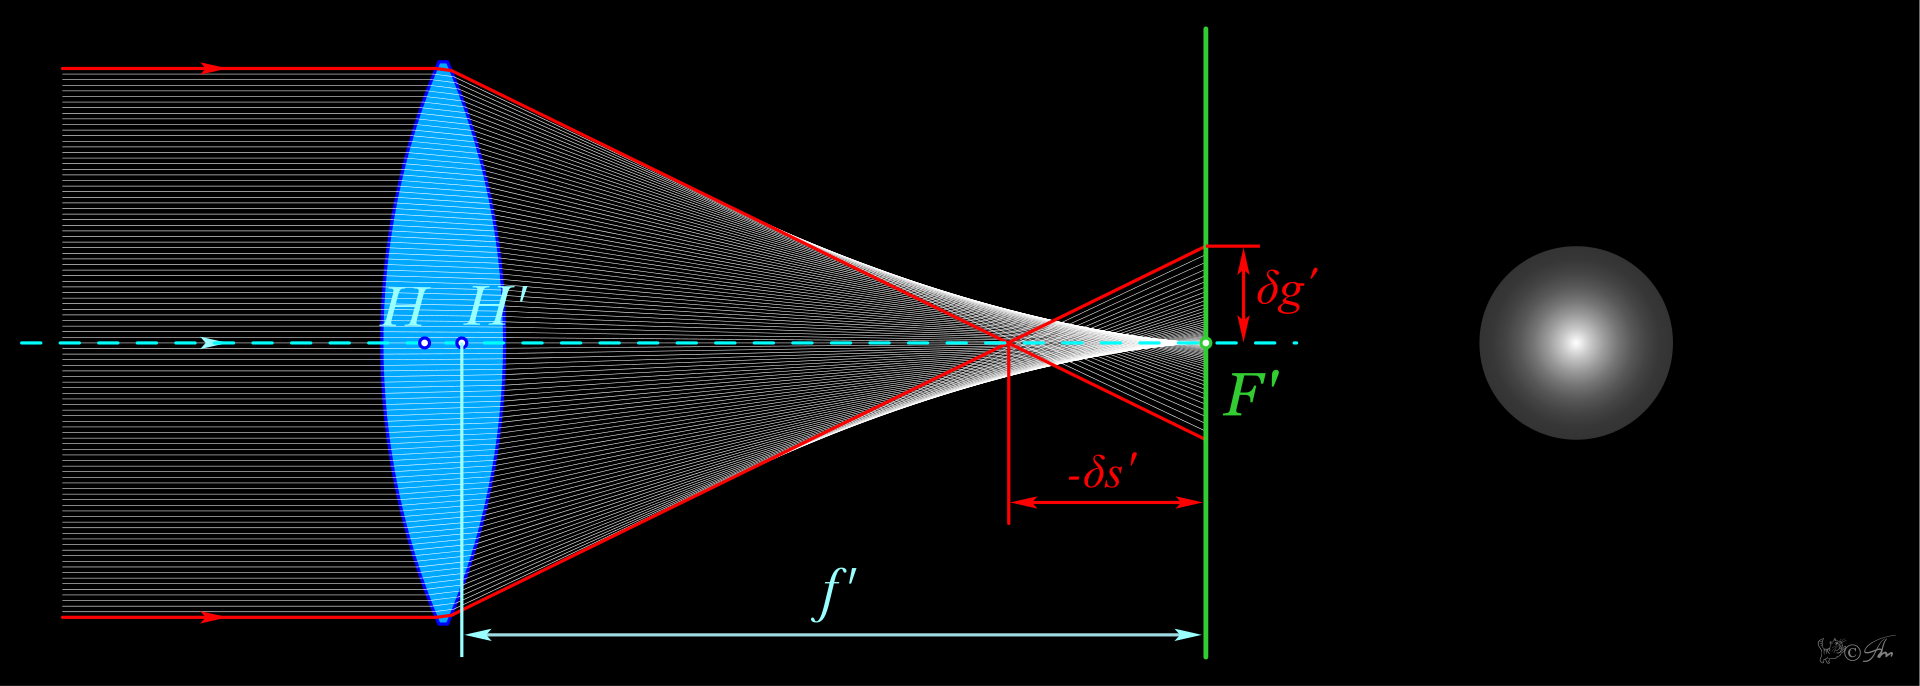
\includegraphics[scale=0.36]{5_sferober.png}
\caption{Схема сферической аберрации, где
	$H$, $H'$ — положения главных плоскостей;
		$F'$  — задняя фокальная плоскость;
		$f'$  — заднее фокусное расстояние;
		$-\delta s'$  — продольная сферическая аберрация;
		$\delta g' = \Delta r'$  — поперечная сферическая аберрация.}
	\label{p1}
	\end{center}
	\end{figure}
	\Def{Сферическая аберрация} — аберрация оптических систем из-за несовпадения фокусов для лучей света, проходящих на разных расстояниях от оптической оси (см. рис.~\ref{p1}.).
ак как сферическая аберрация отвечает члену $A\bm{\sigma}^{2}\bm{\sigma}$, то если в системе есть только этот тип аберрации ($|B|,|C|,|D|,|E|,|F|\approx0\ll |A|$), то
\begin{equation*}
\Delta r'| = A\sigma^{3} = const
\end{equation*} 
 Значит аберрационной кривой является окружность (радиус которой пропорционален кубу входного зрачка), а изображение -- круглое пятнышко, ограниченное этой окружностью (см. рис.1).

\begin{wrapfigure}{r}{0.5\textwidth}
\begin{tikzpicture}
\draw (-2.598,-1.5) arc (210:150:3);
\draw (-2.598,1.5) -- (0,0);
\draw (-2.598,-1.5) -- (0,0);
\draw (-2.598,1.5) -- (0,0);
\draw (-2.598,-1.5) -- (0,0);
\draw (-2.704,1.3) -- (0.2,0);
\draw (-2.704,-1.3) -- (0.2,0);
\draw (-2.791,1.1) -- (0.4,0);
\draw (-2.791,-1.1) -- (0.4,0);
\draw (-2.862,0.9) -- (0.6,0);
\draw (-2.862,-0.9) -- (0.6,0);
\draw (-2.917,0.7) -- (0.8,0);
\draw (-2.917,-0.7) -- (0.8,0);
\draw (-2.958,0.5) -- (1.0,0);
\draw (-2.958,-0.5) -- (1.0,0);
\draw (-2.985,0.3) -- (1.2,0);
\draw (-2.985,-0.3) -- (1.2,0);
\draw (-2.998,0.1) -- (1.4,0);
\draw (-2.998,-0.1) -- (1.4,0);
\end{tikzpicture}
\caption{Каустика -- огибающая лучей от фронта}
\end{wrapfigure}
 В результате сферической аберрации цилиндрический пучок лучей, после преломления линзой (в пространстве изображений) получает вид не конуса, а некоторой воронкообразной фигуры, наружная поверхность которой, вблизи узкого места, называется каустической поверхностью. При этом изображение точки имеет вид диска с неоднородным распределением освещённости, а форма каустической кривой позволяет судить о характере распределения освещённости. В общем случае, фигура рассеяния, при наличии сферической аберрации, представляет собой систему концентрических окружностей с радиусами пропорциональными третьей степени координат на входном (или выходном) зрачке.

\begin{wrapfigure}{r}{0.55\textwidth}
\begin{tikzpicture}[>=latex']
\draw[black] (-2.598,-1.5) arc (210:150:3);
\draw[black] (-2.4,-1.5) arc (-30:30:3);
\draw[black] (-2.4,-1.5) -- (-2.598,-1.5); 
\draw[black] (-2.4,1.5) -- (-2.598,1.5);
\draw[black,->] (-4,-1.2) -- (-3,-1.2);
\draw[black] (-4,-1.2) -- (-2.75,-1.2);
\draw[black,->] (-4,1.2) -- (-3,1.2);
\draw[black] (-4,1.2) -- (-2.75,1.2);
\draw[red,->] (-2.75,1.2) -- (-2.22,1.15);
\draw[green,->] (-2.75,1.2) -- (-2.2,1.1);
\draw[blue,->] (-2.75,1.2) -- (-2.18,1.05);
\draw[red,->] (-2.75,-1.2) -- (-2.22,-1.15);
\draw[green,->] (-2.75,-1.2) -- (-2.2,-1.1);
\draw[blue,->] (-2.75,-1.2) -- (-2.18,-1.05);
\draw[red] (-2.22,1.15) -- (2,0);
\draw[green] (-2.2,1.1) -- (1.5,0);
\draw[blue] (-2.18,1.05) -- (1,0);
\draw[red] (-2.22,-1.15) -- (2,0);
\draw[green] (-2.2,-1.1) -- (1.5,0);
\draw[blue] (-2.18,-1.05) -- (1,0);
\draw[red,->] (-2.22,1.15) -- (-0.11,0.575);
\draw[green,->] (-2.2,1.1) -- (-0.35,0.55);
\draw[blue,->] (-2.18,1.05) -- (-0.59,0.525);
\draw[red,->] (-2.22,-1.15) -- (-0.11,-0.575);
\draw[green,->] (-2.2,-1.1) -- (-0.35,-0.55);
\draw[blue,->] (-2.18,-1.05) -- (-0.59,-0.525);
\draw[gray,dashdotted] (-4,0)--(2.5,0);
\end{tikzpicture}
\caption{Пример хроматической аберрации.}
\label{p3}
\end{wrapfigure} 

Сферическая аберрация линзы (системы линз) объясняется тем, что её преломляющие поверхности встречают отдельные лучи сколько-нибудь широкого пучка под различными углами. Вследствие чего, более удалённые от оптической оси лучи преломляются сильнее, нежели нулевые лучи, и образуют свои точки схода удалённые от фокальной плоскости.
\subsubsection{Хроматическая аберрация}
Если используется белый свет, то в изображении возникают дополнительные аберрации. Это связано с тем, что показатель преломления зависит от длины волны (дисперсия света). Поэтому оптическая система даёт не одно, а множество монохроматических изображений, отличающихся друг от друга по величине и положению. Результирующее же изображение, получающееся от наложения таких монохроматических изображений, оказывается нерезким и с окрашенными краями. Это явление и называется \textit{хроматической аберрацией} (например рис.~\ref{p3}).
\subsection{Коррекция сферической и хроматической аберрации.}
И сферическая и хроматическая аберрации могут быть с той или иной мерой точности откорректированы путём комбинации линз (например, рис.~\ref{p4gl}).
\begin{figure}[H]
	\begin{center}
	\subfigure{\label{p40}}
	\begin{tikzpicture}[>=latex']
	\draw[black] (-2.598,-1.5) arc (210:150:3);
	\draw[black] (-2.4,-1.5) arc (-30:30:3);
	\draw[black] (-2.4,-1.5) -- (-2.598,-1.5); 
	\draw[black] (-2.4,1.5) -- (-2.598,1.5);
	\draw[black,->] (-4,-1.2) -- (-3,-1.2);
	\draw[black] (-4,-1.2) -- (-2.75,-1.2);
	\draw[black,->] (-4,1.2) -- (-3,1.2);
	\draw[black] (-4,1.2) -- (-2.75,1.2);
	\draw[red,->] (-2.75,1.2) -- (-2.22,1.15);
	\draw[green,->] (-2.75,1.2) -- (-2.2,1.1);
	\draw[blue,->] (-2.75,1.2) -- (-2.18,1.05);
	\draw[red,->] (-2.75,-1.2) -- (-2.22,-1.15);
	\draw[green,->] (-2.75,-1.2) -- (-2.2,-1.1);
	\draw[blue,->] (-2.75,-1.2) -- (-2.18,-1.05);
	\draw[red] (-2.22,1.15) -- (2,0);
	\draw[green] (-2.2,1.1) -- (1.5,0);
	\draw[blue] (-2.18,1.05) -- (1,0);
	\draw[red] (-2.22,-1.15) -- (2,0);
	\draw[green] (-2.2,-1.1) -- (1.5,0);
	\draw[blue] (-2.18,-1.05) -- (1,0);
	\draw[red,->] (-2.22,1.15) -- (-0.11,0.575);
	\draw[green,->] (-2.2,1.1) -- (-0.35,0.55);
	\draw[blue,->] (-2.18,1.05) -- (-0.59,0.525);
	\draw[red,->] (-2.22,-1.15) -- (-0.11,-0.575);
	\draw[green,->] (-2.2,-1.1) -- (-0.35,-0.55);
	\draw[blue,->] (-2.18,-1.05) -- (-0.59,-0.525);
	\draw[gray,dashdotted] (-4,0)--(2.5,0);
	\end{tikzpicture}
	\subfigure{\label{p4}}
	\begin{tikzpicture}[>=latex']
	\draw[black] (-2.598,-1.5) arc (210:150:3);
	\draw[black,thick] (-2.4,-1.5) arc (-30:30:3);
	\draw[black] (-2.4,-1.5) -- (-2.598,-1.5); 
	\draw[black] (-2.4,1.5) -- (-2.598,1.5);
	\draw[black,->] (-4,-1.2) -- (-3,-1.2);
	\draw[black] (-4,-1.2) -- (-2.75,-1.2);
	\draw[black,->] (-4,1.2) -- (-3,1.2);
	\draw[black] (-4,1.2) -- (-2.75,1.2);
	\draw[red,->] (-2.75,1.2) -- (-2.22,1.15);
	\draw[green,->] (-2.75,1.2) -- (-2.2,1.1);
	\draw[blue,->] (-2.75,1.2) -- (-2.18,1.05);
	\draw[red,->] (-2.75,-1.2) -- (-2.22,-1.15);
	\draw[green,->] (-2.75,-1.2) -- (-2.2,-1.1);
	\draw[blue,->] (-2.75,-1.2) -- (-2.18,-1.05);
	\draw[black] (-2.4,1.5) -- (-1.6,1.5) -- (-1.6,-1.5) -- (-2.4,-1.5);
	\draw[gray,dashdotted] (-4,0)--(2.5,0);
	%
	\draw[red,->] (-2.22,1.15) -- (-1.6,1.075);
	\draw[green,->] (-2.2,1.1) -- (-1.6,1.05);
	\draw[blue,->] (-2.18,1.05) -- (-1.6,1.03);
	\draw[red,->] (-2.22,-1.15) -- (-1.6,-1.075);
	\draw[green,->] (-2.2,-1.1) -- (-1.6,-1.05);
	\draw[blue,->] (-2.18,-1.05) -- (-1.6,-1.03);
	%
	\draw[red] (-1.6,1.075) -- (2.5,0);
	\draw[green] (-1.6,1.05) -- (2.3,0);
	\draw[blue] (-1.6,1.03) -- (2.1,0);
	\draw[red] (-1.6,-1.075) -- (2.5,0);
	\draw[green] (-1.6,-1.05) -- (2.3,0);
	\draw[blue] (-1.6,-1.03) -- (2.1,0);
	\draw[red,->] (-1.6,1.075) -- (0.45,0.5375);
	\draw[green,->] (-1.6,1.05) -- (0.35,0.525);
	\draw[blue,->] (-1.6,1.03) -- (0.25,0.515);
	\draw[red,->] (-1.6,-1.075) -- (0.45,-0.5375);
	\draw[green,->] (-1.6,-1.05) -- (0.35,-0.525);
	\draw[blue,->] (-1.6,-1.03) -- (0.25,-0.515);
	\end{tikzpicture}
	\end{center}
	\caption{Пример коррекции хроматической аберрации на собирающеё линзе при помощи рассеивающей линзы.}
	\label{p4gl}
\end{figure} 
	
	\newpage
	
	\section{Оптические инструменты. Микроскоп. Телескоп (труба Кеплера, труба Галилея). Угловое увеличение телескопа.}


	
	\newpage
	
	
	\section{Плоская монохроматическая волна. Представление монохроматических волн в
		комплексном виде. Сферическая и цилиндрическая волны. Стоячие электромагнитные
		волны. Опыты Винера.}
	(ЛЛ2 \S 46 и дальше)\\
	\subsection*{Плоские волны}
	Стартуем с обычного волнового уравнения:
	\begin{align*}
	\Delta A - \dfrac{1}{c^2} \dfrac{\partial^2}{\partial t^2}A = 0
	\end{align*}
	Где A - это вектор потенциал, так же помним что такое уравнение было полученно при калибровке $\diver A = 0$. Понятно, что для напряженности электрического и магнитного поля верны такие же уравнения. Хотим изучать плоские волны, это значит, что вектор потенциал может зависить только от одной координаты. Для определенности это x. Тогда уравнение выглядит так:
	\begin{align}
	\dfrac{\partial^2}{\partial x^2}\vec{A} - \dfrac{1}{c^2} \dfrac{\partial^2}{\partial t^2}\vec{A} = 0
	\label{7_1eq}
	\end{align}
	Калибровочное условие превращается в $ \dfrac{\partial}{\partial x}A_x = 0$, значит $\dfrac{\partial^2}{\partial t^2}A_x  = 0$. Отсюда логично заключить, что x компонента потенциала либо линейна по времени, либо ее нет. Первое означало бы наличие постоянного электрического поля, что никакого отношения к волнам не имеет. Значит $A_x = 0$. То есть вектор потенциал всегда лежит в плоскости перпендикулярной направлению движения. Для любого, кто читал конспект по матфизу очевидно, что решением уравнения (\ref{7_1eq}) будет любая функция $\vec{A}(t - \dfrac{x}{c})$ понятно что волна еще может лететь влево, но опустим это, там все то же самое. Из этого решения следует, что 
	\begin{align}
	\dfrac{\partial A}{\partial t} = -\dfrac{1}{c} \dfrac{\partial A}{\partial x}
	\label{7_2eq}
	\end{align}
	Пока запомним это. Теперь вычислим E и H, помня, что вектор потенциал зависит только от x
	\begin{align*}
	\vec{H} = - \vec{e}_y \partial_x A_z + \vec{e}_z \partial_x A_y\\
	\vec{E} = -\dfrac{1}{c} \vec{e}_y\dfrac{\partial A_y}{\partial x} -\dfrac{1}{c} \vec{e}_z \dfrac{\partial A_z}{\partial x}\\
	\vec{E}\vec{H} = -\dfrac{1}{c^2} \partial_x A_y \partial_x A_z +\dfrac{1}{c^2} \partial_x A_y \partial_x A_z = 0
	\end{align*}
	Здесь мы воспользовались формулой (\ref{7_2eq}). Теперь мы знаем, что в любой плоской волне электрическое поле перпендикулярно электрическому. И лежат они в одной плоскости, перпендикулярной направлению распространения волны. Кстати, по модулю они равны, что видно из уравнений выше. Так что можно смело написать:
	\begin{align*}
	S = \dfrac{c}{4\pi} [\vec{E} \vec{H}] = \dfrac{c E^2}{4\pi}\vec{n} = \dfrac{cH^2}{4\pi}\vec{n}
	\end{align*}
	Где вектор n единичный в направлении распространения. \\
	Что такое монохроматическая волна? Это когда $\dfrac{1}{c^2} \dfrac{\partial^2}{\partial t^2}\vec{A} =- \dfrac{\omega^2}{c^2} \vec{A}$, фактически фурье компонента. Если подставить это в уравнение (\ref{7_1eq}), то получим обычное уравнение на гармонический осциллятор для координаты. Значит итоговое решение будет:
	\begin{align*}
	\vec{A} = 	Re\{ \vec{A}_0 e^{-i \omega (t - x/c)}\}
	\end{align*}
	Действительную часть мы взяли потому, что поля не бывают комплексными. А вот $A_0$ бывает. Поэтому правильным выбором $A_0$ волну можно сделать любой комбинацией синусов и косинусов которая нужна. Если взять от этой штуки частную производную по времени, что получить поле не сложно:
	\begin{align*}
	\vec{E} = 	Re\{ \vec{E}_0 e^{-i \omega (t - x/c)}\}
	\end{align*}
	Введя вектор $\vec{k} = \dfrac{\omega}{c} \vec{n}$ можно отвязаться от координат и просто написать
	\begin{align*}
	\vec{E} = 	Re\{ \vec{E}_0 e^{i (kr - \omega t)}\}
	\end{align*}Понятие о когерентности. Частично когерентный свет. Основные интерференционные
	схемы. Интерференция плоских волн, пространственный период полос.
	Обычно взятие действительной части опускают. Так пока мы совершаем линейные операции с полями нам это не важною.  \\
	\subsection*{Сферические и цилиндрические волны}
	Для простоты рассмотрим только монохроматические. Сферические волны это когда зависимость есть только от расстояния до начала координат. Вспоминая как вылгядит оператор лапласа в сферике (например в вики) и быстро решая уравнение получаем (Re опустил):
	\begin{align*}
	A = A_0 \dfrac{e^{i (kr - \omega t)}}{r}
	\end{align*}
	Теперь пишем дифур на цилиндрические волны. \textbf{Здесь r - расстояние до оси}
	\begin{align*}
	&\dfrac{1}{r} \partial_r (r \partial_r f) + k^2 f = 0\\
	& x = r k\\
	&f'' + \dfrac{1}{x} f' + f = 0
	\end{align*} 
	А это уравнение на функцию Бесселя. Конечно есть еще функция Неймана, но нам надо чтобы в нуле значение было конечным, а функция Неймана этого не дает. Итого решениe пропорцианально такой штуке: $J_0(k r) e^{-i\omega t}$ на больших временах можно написать асиптотику: 
	\begin{align*}
	A_0 \dfrac{e^{i (kr - \omega t - \pi/4)}}{\sqrt{r}}
	\end{align*}
	\subsection*{Стоячие волны и опыт Винера}
	Если есть две одинаковые волны $e^{i (kr - \omega t)} \quad e^{i (-kr - \omega t)}$, идущие в разных направлениях (например после отражения), то их можно сложить и получить $2\cos \omega t \cos k r$\\
	Но физически мы можем заметить только квадрат амплитуды. Ну тут видно, что после усреднения по времени мы будем наблюдать серию кучностей на расстоянии по $\lambda/2$ друг от друга. Проблема в их наблюдении это малая длина волны. Вот что придумал Винер.\\
	Берем фоточувствительную пластинку и ставим ее под малым углом к зеркалу. Освещаем зеркало монохроматическим светом на наблюдаем тучности непосредственно
	\begin{figure}[H]
		\centering
		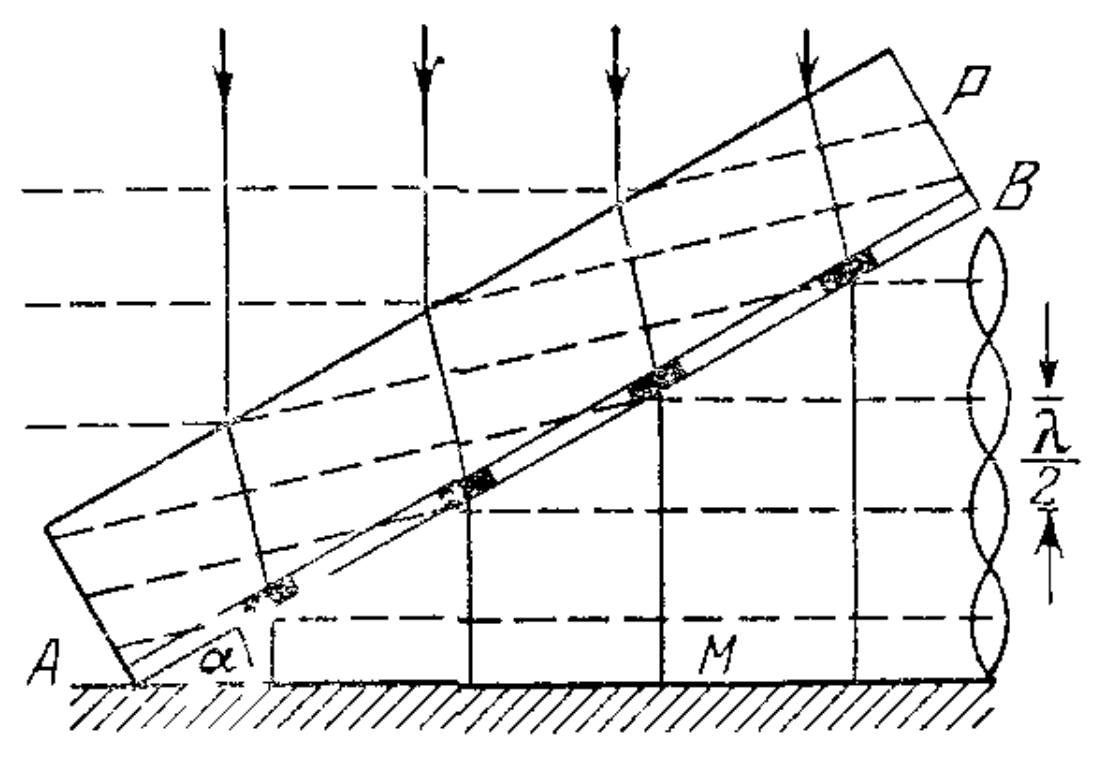
\includegraphics[scale = 0.3]{7_1}
	\end{figure}
	Расстояние между ними по прямой будет $\dfrac{\lambda}{2 \sin \alpha}$, то есть зная синус наклона можно узнать и длину волны.  
	
	\newpage
	
	\input{TeX_files/8.tex}
	
	\newpage
	
	\input{TeX_files/9.tex}
	
	\newpage
	
	\input{TeX_files/10.tex}
	
	\newpage
	
	\section{Оптические явления на границе раздела изотропных диэлектриков. Соотношения амплитуд падающей, отраженной и преломленной волн (формулы Френеля). Изменение фазы волны при отражении. Энергетические коэффициенты отражения и пропускания света. Коэффициент отражения для естественного света.}

% Дописать про изменение фазы волны при отражении -- вроде бы было в Овчинкине (семинары)?

% Коэффициент отражения -- ?????

При падении плоской волны на границу раздела двух изотропных диэлектриков, появляется две волны: преломленная (которая проходит границу раздела сред) и отраженная (не проходит), которые создаются за счет колебаний в диэлектриках, возбуждаемых падающей волной. Сразу быстро получим законы отражения и преломления.

\subsection{Законы отражения и преломления}

Пусть падающая волна имеет следующий вид:

\begin{equation*}
\vec{E} = \vec{E}_0 \cdot e^{-i (\omega t - \vec{k} \cdot r)}
\end{equation*}

В таком случае, из-за того, что колебания являются вынужденными, мы можем сказать, что $\omega = \omega_r = \omega_t$.

Кроме того, как мы знаем из курса электричества, существует уравнение на граничное условие для вектора $E$, которое в нашем случае принимает вид (для тангенциальных компонент):

\begin{equation*}
E_\tau + E_{r\tau} = E_{t\tau}
\end{equation*}

Возьмем любую точку на линии границы сред. В таком случае:

\begin{equation*}
A_1 e^{i \vec{k} \vec{x}} + B_1 e^{i \vec{k}_r \vec{x}} = C_1 e^{i \vec{k}_t \vec{x}}
\end{equation*}

Это в свою очередь значит, что должны быть равны между собой величины, стоящие в показателе экспоненты. С учетом того, как мы ввели углы, получаем:

\begin{equation}
k\sin\phi = k_r \sin \phi_r = k_t \sin\phi_t
\label{eq:reflection_and_refraction}
\end{equation}

При этом, как мы знаем, $k$ зависит от свойств среды, поэтому для падающей волны и отраженной:

\begin{equation*}
k = k_r = \frac{w}{c} \sqrt{\mu \epsilon}
\end{equation*}

А для преломленной:

\begin{equation*}
k_t = \frac{w}{c} \sqrt{\mu'\epsilon'}
\end{equation*}

Тогда из уравнения \ref{eq:reflection_and_refraction} получаем:

\begin{align*}
&\phi = \phi_r\\
&\frac{\sin\phi_t}{\sin\phi} = \frac{k}{k_t} = \frac{\sqrt{\epsilon\mu}}{\sqrt{\epsilon'\mu'}} = \frac{n}{n'}
\end{align*}

\subsection{Коэффициенты Френеля}

Разложим падающую волну $\vec{E}$ по двум составляющим: в плоскости, параллельной плоскости рисунка, и в плоскости, перпендикулярной ($E_\parallel$ и $E_\perp$ соответственно). Мы имеем следующие граничные условия:

\begin{align*}
&E_\tau + E_{r\tau} = E_{t\tau}\\
&H_\tau + H_{r\tau} = H_{t\tau}
\end{align*}

Мы также знаем соотношение, связывающее между собой $H$ и $E$: $H = \sqrt{\epsilon}E$ (пренебрегаем магнитными свойствами сред и считаем $\mu = 1$, а также не забываем, что $\vec{H} \perp \vec{E}$). Также вспоминаем, что $n = \sqrt{\epsilon}$. Тогда граничные условия принимают вид (с учетом проекций, см. рисунок): % Вставить рисунок

\begin{align*}
&\begin{cases}
&E\cos\phi_1 - E_r\cos\phi_1 = E_t\cos\phi_2\\
&n_1 E + n_1 E_r = n_2 E_t\\
&\dfrac{\sin\phi_1}{\sin\phi_2} = \dfrac{n_2}{n_1}
\end{cases}
\quad &\text{--- для параллельной}\\
&\begin{cases}
&E - E_r = E_t\\
&n_1 E \cos\phi_1 + n_1 E_r \cos\phi_1 = n_2 E_t \cos\phi_2\\
&\dfrac{\sin\phi_1}{\sin\phi_2} = \dfrac{n_2}{n_1}
\end{cases}
\quad &\text{--- для перпендикулярной}\\
\end{align*}

Решив эту систему уравнений, мы получаем следующее:

\begin{align*}
&\begin{cases*}
E_r = \dfrac{\tg(\phi_1 - \phi_2)}{\tg(\phi_1 + \phi_2)}E\\
E_t = \dfrac{2\sin\phi_2\cos\phi_1}{\sin(\phi_1 + \phi_2) \cos(\phi_1 - \phi_2)}E
\end{cases*}
\quad &\text{--- для параллелльной}\\
&\begin{cases*}
E_r = \dfrac{\sin(\phi_2 - \phi_1)}{\sin(\phi_1 + \phi_2)}E\\
E_t = \dfrac{2\sin\phi_2\cos\phi_1}{\sin(\phi_1 + \phi_2)}E
\end{cases*}
\quad &\text{--- для перпендикулярной}
\end{align*}

Можно сразу же ввести энергетические коэффициенты отражения и пропускания света:

\begin{align*}
R_\parallel = \left(\frac{E_r}{E}\right)^2 = \frac{\tg^2\left(\phi_1 - \phi_2\right)}{\tg^2(\phi_1 + \phi_2)} \qquad T_\parallel = 1 - R_\parallel\\
R_\perp = \left(\frac{E_\perp}{E}\right)^2 = \frac{\sin^2(\phi_2 - \phi_1)}{\sin^2(\phi_2 + \phi_1)} \qquad T_\perp = 1 - R_\perp
\end{align*}
	
	\newpage
	
	\input{TeX_files/12.tex}
	
	\newpage
	
	\input{TeX_files/13.tex}
	
	\newpage
	
	\input{TeX_files/14.tex}
	
	\newpage
	
	\input{TeX_files/15.tex}
	
	\newpage
	
	\section{Принцип суперпозиции и интерференция монохроматических волн. Интерференция плоской и сферической волн. Видность полос.}

\theornp{Принцип суперпозиции}{Если в одной точке пространства накладываются колебания двух волн, то они порождают новую волну, равную их векторной сумме.}

Из-за наличия принципа суперпозиции возможно явление интерференции, когда волны взаимно усиляют друг друга, или же наоборот, гасят.

\Def{Монохроматическая волна} --- волна, в спектр которой входит только одна частота.

\subsection{Интерференция двух плоских монохроматических волн. Ширина полосы}

Рассмотрим сперва интерференцию двух плоских монохроматических волн. Пусть распространяются две волны с одинаковой частотой $\omega$:

\begin{align*}
	E_1 &= a_1 e^{i(\vec{k}\cdot \vec{r}_1 - \phi_1)} \cdot e^{-i\omega t}\\
	E_2 &= a_2 e^{i(\vec{k}\cdot \vec{r}_2 - \phi_2)} \cdot e^{-i\omega t}
\end{align*}

Как мы знаем, сами по себе волны складываются. Посмотрим теперь за интенсивностью $I$, которую мы запишем как $I = E E^*$. Распишем суммарную интенсивность (принимаем во внимание, что временная часть в экспоненте одинаковая у всех, поэтому она сократится при произведении с комплексно сопряженным и поэтому следить за ней не будем):

\begin{align*}
	I_{\sum} = (E_1 + E_2) (E_1 + E_2)^* = E_1 E_1^* + E_1 E_2^* + E_2 E_1^* + E_2 E_2^* = \\
	= a_1^2 + 2 a_1 a_2 \cos(k \Delta - \Delta\phi) + a_2^2 = I_1 + I_2 + 2 \sqrt{I_1 I_2} \cos(k \Delta - \Delta\phi)
\end{align*}

Здесь мы ввели $\Delta = r_2 - r_1$, $\Delta\phi = \phi_2 - \phi_1$. Напоминаю, что $k = 2\pi / \lambda$.

\textit{Если же $k_1 \ne k_2$, то вместо $k$ в результирующей формуле будет $K = |k_1 - k_2|$.}

\subsubsection{Ширина полосы}

Рассмотрим чуть более общий случай, когда $|k_1| = |k_2|$, но при этом волны сходятся под некоторым углом $\alpha$. Тогда $K = 2 k \sin(\alpha/2)$

\textbf{Шириной полосы} будем называть расстояние между ближайшими максимумами (\textit{вообще говоря, в МФТИшном конспекте написано что между минимумами, а между максимумами это расстояние между полосами, но наш лектор видимо так не считает, но строго говоря какая разница казалось бы}). В нашем случае она оказывается равной:

\begin{equation*}
	\Delta x = \frac{2\pi}{K} = \frac{2 \pi}{2 k \sin(\alpha/2)} = \frac{\lambda}{2\sin(\alpha/2)} \approx \frac{\lambda}{\alpha}
\end{equation*}

\subsection{Интерференция плоской и сферической монохроматических волн}

Внимание на картинку. % Вставить картинку.

Будем рассматривать область, где $R_0 \gg r$. При этом:

\begin{equation*}
	R = \sqrt{R_0 + r^2} \approx R_0 + \frac{r^2}{2R_0}
\end{equation*}

Для сферической волны:

\begin{equation*}
	E_{sp} = \frac{a_1}{R_0} e^{i k r} e^{-i \omega t} \approx \frac{a_1}{R_0} e^{i k (R_0 + r^2 / (2 R_0))} e^{-i \omega t}
\end{equation*}

Для плоской волны:

\begin{equation*}
	E_{f} = a_2 e^{i k R_0  - i \omega t}
\end{equation*}

Если это счастье расписать так же, как мы делали с плоской волной, то получим:

\begin{equation*}
	I_{\sum} = \frac{a_1^2}{R_0^2} + a_2^2  + 2 \frac{a_1 a_2}{R_0} \cos \left(k \frac{r^2}{2 R_0}\right)
\end{equation*}

\subsection{Видность}

Для характеристики выраженности интерференции вводят величину, называемую \textbf{видностью} $V$:

\begin{equation}
	V = \frac{I_{max} - I_{min}}{I_{max} + I_{min}}
	\label{eq:Vidnost}
\end{equation}

где $I_{max}$, $I_{min}$ --- максимальное и минимальное значения интенсивности в области интерференции волн.

При интерференции двух \textbf{монохроматических} волн видность будет равна:

\begin{equation*}
	V = \frac{2 \sqrt{I_1 I_2}}{I_1 + I_2}
\end{equation*}
	
	\newpage
	
	\input{TeX_files/17.tex}
	
	\newpage
	
	\input{TeX_files/18.tex}
	
	\newpage
	
	\input{TeX_files/19.tex}
	
	\newpage
	
	\input{TeX_files/20.tex}
	
	\newpage
	
	\section{Пространственная когерентность. Интерференция квазимонохроматических волн протяженных источников света. Роль конечных размеров источника света. Интерференционная картина в схеме Юнга.}
	
	\newpage
	
	\input{TeX_files/22.tex}
	
	\newpage
	
	\input{TeX_files/23.tex}
	
	\newpage
	
	\input{TeX_files/24.tex}
	
	\newpage
	
	\input{TeX_files/25.tex}
	
	\newpage
	
	\section{Интерферометр Майкельсона. Фурье-спектрометр. Применение интерферометров в научных исследованиях}

\subsection{Интерферометр Майкельсона}

Схема интерферометра представлена на рисунке. % Сюда нужен рисунок.
Приведем краткое описание:

Свет от некоторого протяженного источника $S$ попадает на плоскопараллельную полупрозрачную пластинку $P_1$. Она разделает попавший на нее пучок на два, первый и второй соответственно. Первый пучок, после прохождения пластинки, отражается обратно \textbf{статичным} зеркалом $M_1$, после чего частично отражается от пластинки $P_1$ в указанном направлении. Второй же пучок, отразившись от границы пластинки $P_1$, направляется к зеркалу $M_2$, после чего проходит через пластинку $P_1$ и идет совместно с пучком 1. Отметим, что второй пучок проходит пластину $P_1$ трижды. Чтобы исключить получающуюся из-за этого разность фаз, на пути первого пучка ставят пластинку $P_2$, идентичную $P_1$.

Пусть $M_1'$ --- изображение зеркала $M_1$ в отражающей плоскости пластинки $P_1$. Тогда происходящая интерференция равносильна интерференции в воздушном слое между $M_1'$ и $M_2$. Разность хода между лучами составляет $\Delta = 2 d\cos \phi$, где $d$ --- толщина слоя, $\phi$ --- угол падения. Если слой плоскопараллелен, то мы получим интерференционные кольца с центром в точке схождения лучей, нормально отраженных от поверхностей $M_1'$ и $M_2$. Этому направлению соответствует максимальная разность хода $\Delta = 2 d$, значит максимальный порядок интерференции будет в центре. При увеличении $d$ полосы будут перемещаться от центра; при увеличении зазора на $d = \lambda/2$, произойдет смещение картины на одну полосу (т.е. на место светлой полосы снова придет светлая), т.к. $\Delta = \lambda$. Если же мы измени угол падения, то разность хода изменится на $\Delta = 2 d \sin\phi \Delta\phi$. Полосы получаются чем шире, чем меньше $d$, т.е. при $d = 0$ мы получим равномерное освещение.

Интерферометр использовался, например, при проведении  \href{https://elementy.ru/trefil/21167/Opyt_MaykelsonaMorli}{опыта Майкельсона -- Морли}, в ходе которого было установлено отсутствие движения Земли относительно эфира.

\subsection{Фурье-спектрометр}

Схема спектрометра представлена на рисунке. Приведем краткое описание: % Сюда тоже нужна картинка.

Основой спектрометра является интерферометр Майкельсона (только он тут почему-то без второй пластины, ха-ха). Предположим, что у нас есть некоторый когерентный источник излучения с длиной волны $\lambda$. Когда разность хода лучей в спектрометре оказывается равной $\lambda/2$, интенсивность регистрируемого света оказывается близкой к нулю. При перемещении правого зеркала интерферометра Майкельсона разность хода лучей изменяется, изменяется и интенсивность света, регистрируемая приёмником. Очевидно, что интенсивность света максимальная, когда разность хода лучей будет кратна длине волны $\lambda$.

При перемещении зеркала с постоянной скоростью на выходе приёмника будет наблюдаться электрический сигнал синусоидальной формы. Притом период синусоиды зависит от длины волны источника, а амплитуда от интенсивности источника.

Теперь представим, что на входе некогерентный источник. Каждая длина волны в спектре источника света будет давать свою синусоиду на выходе приёмника. Таким образом, на выходе приёмника мы получаем сложный сигнал. При выполнении над полученным сигналом обратного преобразования Фурье получаем спектр входного электрического сигнала, который также является спектром излучения источника (то есть интенсивность излучения источника на различных длинах волн).

За счет этого можно проводить спектральные анализы для выявления состава газов или жидкостей. Каждый газ или жидкость имеет свой спектр поглощения проходящего через него излучения. Таким образом спектр на входе интерферометра будет иметь «провалы» на определённых длинах волн. После обратного преобразования Фурье получаем спектр поглощения, по которому достаточно просто определить присутствующие в анализируемом воздухе газы и их концентрацию.

\subsection{Применение интерферометров в научных исследованиях}

Фактически, интерферометр позволяет с большой точностью измерять расстояния, поэтому его можно применять для создания деталей, изготовление которых требует высокой точности (сдвиг в интерференционной картине будет виден даже при небольшом отклонении).

Интерференционные методы позволяют с высокой точностью выявлять очень малые изменения показателя преломления среды, которые влияют на изменение оптической длины пути, а значит, влекут за собой изменение интерференционной картины.

Можно также измерять и углы.
	
	\newpage
	
	\input{TeX_files/27.tex}
	
	\newpage
	
	\input{TeX_files/28.tex}
	
	\newpage
	
	\input{TeX_files/29.tex}
	
	\newpage
	
	\input{TeX_files/30.tex}
	
	\newpage
	
	\section{Дифракция Френеля на прямолинейном краю плоского экрана и щели. Зоны Шустера, спираль Корню.}
	
	\newpage
	
	\input{TeX_files/32.tex}
	
	\newpage
	
	\input{TeX_files/33.tex}
	
	\newpage
	
	\input{TeX_files/34.tex}
	
	\newpage
	
	\input{TeX_files/35.tex}
	
	\newpage
	
	\section{Роль дифракции в приборах, формирующих изображение. Критерий Рэлея (применительно к формированию изображений). Дифракционный предел разрешения телескопа и микроскопа.}

Из-за наличия во Вселенной дифракции Фраунгофера на круглом отверстии, вместо точки при фокусировке света мы получаем небольшое пятнышко, которое называется \textbf{пятном (диском) Эйри}. Его радиус можно рассчитать по следующей формуле:

\begin{equation*}
	\rho_{a} = 1.22 \frac{\lambda}{D} F	
\end{equation*}

Здесь $\lambda$ --- длина волны наблюдаемого излучения, $D$ --- диаметр линзы, $F$ --- ее фокусное расстояние.

Пусть мы наблюдаем некоторый объект, который находится на главной оптической оси. Тогда и его изображение будет находиться там же. Пусть теперь у нас добавляется еще один объект, который находится от первоначального на некотором (небольшом) угловом расстоянии $\psi$. Пятно Эйри от этого объекта в таком случае будет находиться на таком же угловом расстоянии от исходного пятна, а линейное расстояние тогда будет равно $l = F \psi$. 

Для того, чтобы понять, возможно ли эти два объекта разрешить, был введен так называемый \textbf{критерий Рэлея}, который говорит, что минимальное расстояние между объектами, на котором их можно разрешить, оказывается таким, что первый минимум пятна Эйри от одного объекта приходится на нулевой максимум пятна Эйри другого (см рисунок) % Вставить рисунок.

С учетом имеющейся у нас формулы для радиуса пятна Эйри мы получим:

\begin{equation*}
	\psi_{min} F = 1.22 \frac{\lambda}{D} F \qrq \boxed{\psi_{min} = 1.22 \frac{\lambda}{D}}
\end{equation*}

Рассмотрим теперь микроскоп. Предположим, что предмет у нас лежит в какой-то среде с показателем преломления $n$ (так делается, например, в диффузионных микроскопах); по другую сторону линзы у нас, соответственно, воздух, с показателем преломления $n_{air} = 1$. Как уже было сказано ранее, от каждой точки предмета будет получаться не точечное изображение, а пятно Эйри. Введем углы $u_1$ и $u_2$ (см. рисунок). Угол $u_1$ называется апертурным углом объектива. % Вставить рисунок.

Как видно из рисунка, верно следующее:

\begin{equation*}
	\frac{D}{L} \approx 2 u_2 \approx 2 \sin u_2
\end{equation*}

Согласно Аббе, идеальный с точки зрения геометрии микроскоп подчиняется следующему условию (\textbf{условие синусов Аббе}):

\begin{equation*}
	l_1 n_1 \sin u_1 = l_2 n_2 \sin u_2 \qrq l_1 n \sin u_1 = l_2 \frac{D}{2L}
\end{equation*}

Здесь $l_1$ и $l_2$ есть линейные размеры предмета и изображения соответственно.

Ну и с учетом критерия Рэлея, который в данном случае удобно сформулировать как "линейный размер изображения должен получаться не меньше радиуса пятна Эйри", мы получим:

\begin{equation*}
	l_{2 min} = \rho_a = l_{1 min} \frac{2 L n\sin u_1}{D} = 1.22 \frac{\lambda}{D} L \qrq l_{1 min} = 0.61 \frac{\lambda}{n\sin u_1}
\end{equation*}

Выражение $n \sin u_1$ в знаменателе называют \textbf{числовой апертурой микроскопа}.
	
	\newpage
	
	\input{TeX_files/37.tex}
	
	\newpage
	
	\input{TeX_files/38.tex}
	
	\newpage
	
	\input{TeX_files/39.tex}
	
	\newpage
	
	\input{TeX_files/40.tex}
	
	\newpage
	
	\section{Зависимости показателя преломления и коэффициента поглощения от частоты. Дисперсионная формула Зелмеера. Фазовая и групповая скорости. Формула Рэлея.}
	
	\newpage
	
	\input{TeX_files/42.tex}
	
	\newpage
	
	\input{TeX_files/43.tex}
	
	\newpage
	
	\input{TeX_files/44.tex}
	
	\newpage
	
	\input{TeX_files/45.tex}
	
	\newpage
	
	\section{Модель двухуровневой системы Взаимодействие двухуровневой системы с излучением: спонтанные и вынужденные переходы. Коэффициенты Эйнштейна. Многоуровневые системы.}
	
	\newpage
	
	\input{TeX_files/47.tex}
	
	\newpage
	
	\input{TeX_files/48.tex}
	
	\newpage
	
	\input{TeX_files/49.tex}
	
	\newpage
	
	\input{TeX_files/50.tex}
	
	
	
	
	
	
	
	
	
	
	
	
\end{document}